% !TeX root = ../../thesis.tex


%overview of the methodology to be used;
% ~20 pages

\chapter{Methodology}
\label{chap:methods}

A number of studies related to this thesis have been reviewed in Chapter \ref{chap:rw}. This chapter discusses why the semantic web will be used for linking sensor metadata and which methods will be used to achieve this. The \ac{swe} standards, the om-lite and sam-lite ontologies, and \ac{rdf} will be described. Also a brief overview of the data use for this thesis is presented.   

\section{Sensor metadata on the semantic web}
\ac{semsos} \citep{SSW:Henson, SSW:Pschorr} as well as \ac{sel} \citep{SSW:Janowicz} focus on combining the sensor web with the semantic web, but do not address the integration and aggregation of sensor data. Similarly, \cite{SSW:Atkinson} proposes to expose sensor data to the semantic web in order to find other kinds of related data about the same feature-of-interest. Data that can be collected for another area of research. However, \cite{SSW:Atkinson} do not mention the integration of complementary sensor data from heterogeneous sources either. \cite{SSW:Stasch} and \cite{SSW:Stasch3} suggest interesting methods for aggregating sensor data based on features-of-interest. However, also these studies use sensor data from only a single source into account. Moreover, \cite{SSW:Corcho} and \cite{SSW:Ji} argue that methods for integration and fusion of sensor data on the semantic web is still an area for future research. Data fusion is \enquote{a data processing technique that associates, combines, aggregates, and integrates data from different sources} \cite[p. 2]{SSW:Wang2}. 

\cite{SW:OGC3} and \cite{SW:OGC4} present methods for including \ac{sos} services in an \ac{ogc} catalogue service using \ac{sor} and \ac{sir}. Making sensor metadata available in a catalogue service will improve the discovery. However, discovery through the semantic web is likely to be more effective, since links can be created towards the sensor data from many different sources of related information. Another advantage is that links can be created by everybody that publishes linked data on the web, allowing sensor data to be used for implementations that were not identified beforehand by the publisher. Also, the semantic web will be easier to access, while the catalogue service can only be requested at a certain \ac{url} which has to be known to potential users. 

Since data on the web has a distributed nature it can be questioned whether centralised catalogue services are feasible to create. It places a burden on the owner of the \ac{sos} to register with a catalogue service. Also, there could be multiple of these services on the web creating issue regarding the discovery of relevant catalogues. The semantic web could solve this issue by getting rid of the `dataset-centric' approach and adding metadata directly to the web instead.

\section{Semantic Web and the Internet of Things}
\cite{IOT:Barnaghi} describe how the semantic web could be of great importance for the \ac{iot}.
\cite{IOT:Jazayeri} describe the \ac{sos} as one of the protocols that \ac{iot} devices could use.

\section{Creating linked data}
For publishing sensor data on the semantic web a conversion of this data to \ac{rdf} is required. For this the method by \cite{LD:Missier} will be used. She developed a workflow for publishing linked open data, using existing spatial data as input (Figure \ref{fig:missier}). This workflow consists of three phases: preparation, modelling and conversion. The next paragraphs will describe these three phases in more detail.

\begin{figure}
	\centering
	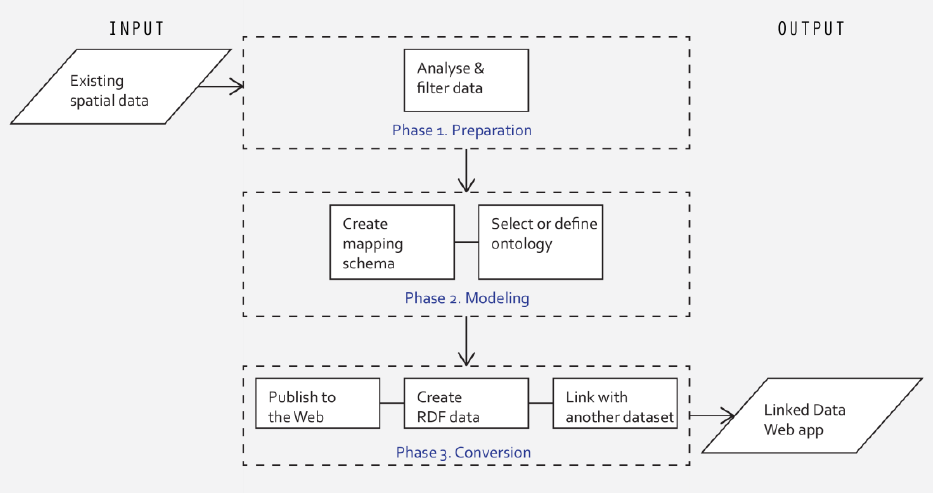
\includegraphics[width=1\linewidth]{UML/workflowMissier.png}
	\caption{Workflow diagram for publishing linked open data from existing spatial data \citep[p. 28]{LD:Missier}}
	\label{fig:missier}
\end{figure}

\subsection{Preparation}
The preparation phase deals with data acquisition, analysis and filtering. After an acquired dataset has been selected to convert to linked data it should be carefully examined. When creating linked data it is important to know the content and format of the input data. \cite{LD:Missier} explains that this understanding of the data is crucial for selecting the right ontologies and using the right software tools to process the data. Data filtering should be performed to select the parts of the dataset that need to be mapped to linked data. In this step the data quality could also be improved if necessary. The result of this phase should be a clean dataset, with semantics about the content, which has been filtered to only contain the parts of data that are required as linked data. 
 
\subsection{Modelling}
The first step in modelling data to linked data is to select an ontology. An ontology is part of a data model, that contains semantics of how objects in the real world are mapped inside a dataset. To improve interoperability is preferred to (re)use an already existing ontology. However, if there is no suitable ontology available a new one should be created. To select an ontology all ontologies that describe the type of data inside the dataset should be listed. The one that fits the dataset and the final application best should be selected from these ontologies. \cite{LD:Missier} stresses that it is also important to reuse common predicates associated with an ontology. This makes the data more understandable and it is easier to merge with other datasets using the same ontology and predicate. 

 
\subsection{Conversion}


\section{Spatial Queries with SPARQL}
\label{par:SpatialFilters}
GeoSPARQL \enquote{defines a vocabulary for representing geospatial data in RDF, and it defines an extension to the SPARQL query language for processing geospatial data} \cite[p. xvi]{LD:OGC}. It allows for defining geometric data in \ac{rdf} and performing spatial queries. The \ac{DE9IM} \citep{GIS:9IM} has been implemented to find topological relations between two geometries. GeoSPARQL has been implemented in the `Parliament' \ac{sparql} endpoint \citep{LD:GeoSPARQL}. The Strabon endpoint uses stRDF, which is \enquote{a constraint data model that extends RDF with the ability to represent spatial and temporal data} \cite[p. 425]{SSW:Koubarakis}. The stRDF model can be queried using stSPARQL, which syntax is similar to GeoSPARQL (listing \ref{lst:GeoSPARQL} \& \ref{lst:stSPARQL}). Both extensions of \ac{sparql} use filter expressions to perform spatial operations on \ac{wkt} or \ac{gml} geometries. The definition of geometries and the syntax of the filter expression differ slightly.

\begin{lstlisting}[caption={A GeoSPARQL query to find the names of features that contain a point geometry}, label={lst:GeoSPARQL}]
PREFIX geo: <http://www.opengis.net/ont/geosparql#>
PREFIX geof: <http://www.opengis.net/def/function/geosparql/>
PREFIX foaf: <http://xmlns.com/foaf/0.1/> 

SELECT 
?name
WHERE {
?feature geo:hasGeometry ?geom .
?feature foaf:name ?name.
FILTER (geof:sfContains(?geom,"<http://www.opengis.net/def/crs/EPSG/0/4258> POINT(4.289244 52.027337)"^^geo:wktLiteral))
}
\end{lstlisting}

\begin{lstlisting}[caption={A stSPARQL query to find the names of features that contain a point geometry}, label={lst:stSPARQL}]
PREFIX strdf: <ttp://strdf.di.uoa.gr/ontology#>
PREFIX foaf: <http://xmlns.com/foaf/0.1/> 

SELECT 
?name
WHERE {
?feature strdf:hasGeometry ?geom .
?feature foaf:name ?name.
FILTER (?geom contains "POINT(4.289244 52.027337);<http://www.opengis.net/def/crs/EPSG/0/4258>"^^strdf:WKT)
}
\end{lstlisting}

\section{Ontologies}
When publishing data on the semantic web, ontologies are required to specify what things are and how they relate to other things. The evaluation of observation metadata ontologies by \cite{SW:Hu} is interesting, since it exposes what the relevant aspects are in the process of observation discovery. However, their proposed model focusses mainly on including remote sensing and imagery data in metadata models that were not originally created for this kind of data. The \ac{ssno} is an ontology that clearly describes the process between sensor, stimulus and observation. However, \cite{SSW:Cox4} points out that an important aspect of describing a sensor network is missing in this ontology: the sampling. Also, the om-lite and sam-lite ontologies by \cite{SSW:Cox4} are lightweight ontologies that can be complemented by already existing linked data ontologies. They do not rely on the (heavy) \ac{iso} specifications that date from before the semantic web, unlike the \ac{ssno}. The om-lite and sam-lite ontologies will therefore be used in this thesis. 

The \ac{sos} has a number of metadata attributes such as the service provider's details (including contact information), its spatial and temporal extent (spatialFiler \& temporalFilter) and the capabilities to query a subset of this extent. It receives data from a sensor which makes observations. An observation can be defined as \enquote{an action whose result is an estimate of the value of some property of the feature-of-interest, obtained using a specified procedure} \citep{SSW:Cox3}.The sensor is placed at a sampling point. The sampling point is part of a sampling feature which intents to resemble the feature-of-interest. In the case of air quality the feature-of-interest is the bubble of air surrounding the sensor, therefore the sampling point equals the feature-of-interest \citep{SDI:INSPIRE2}. The design is that an observation of the sampling feature describes the  feature-of-interest through measuring one of its properties. The measurement procedure is described by a short string of text, input and output parameters and the units of measurement of the ouput. The relation between feature-of-interest and administrative units is added to improve the discovery of sensor data on the semantic web. 

To publish data on the semantic web ontologies are required to specify the different classes and their relations. An ontology for static geographic data has to be connected to an ontology for sensor metadata. From the \ac{uml} diagram in Figure \ref{fig:UML} the classes Observation, Process, ObservedProperty and FeatureOfInterest can be mapped to classes belonging to \ac{owl} for observations \citep{SSW:Cox}. SamplingFeature and Sampling point can be mapped to classes from \ac{owl} for sampling features \citep{SSW:Cox2}. GeoSPARQL can be used for the administrativeUnit class \citep{LD:OGC} and the PROV ontology for the sensor and sensor observation service classes \citep{LD:W3C2}. 


\section{Web Processing Service}
The \ac{ogc} \acl{wps} is a standard interface for making simple or complex computational processing services accessible as web services. Originally, it has been created with spatial processes in mind, but it can also be used to insert non-spatial processing into a web services environment \citep[p. 8]{GEO:OGC}. Via the \ac{wps} jobs can be controlled and monitored, which run certain processes (Figure \ref{fig:WPSmodel}). Similar to \ac{wfs}, \ac{wps} and \ac{sos}, the \ac{wps} has requests for retrieving metadata: \texttt{GetCapabilities} and \texttt{DescribeProcess}. On top of that there are is the \texttt{Execute} request to execute a process, and a number of other requests for various purposes: \texttt{GetStatus}, \texttt{GetResult} and \texttt{Dismiss}. All requests will be briefly described in this paragraph.  

\begin{figure}
	\centering
	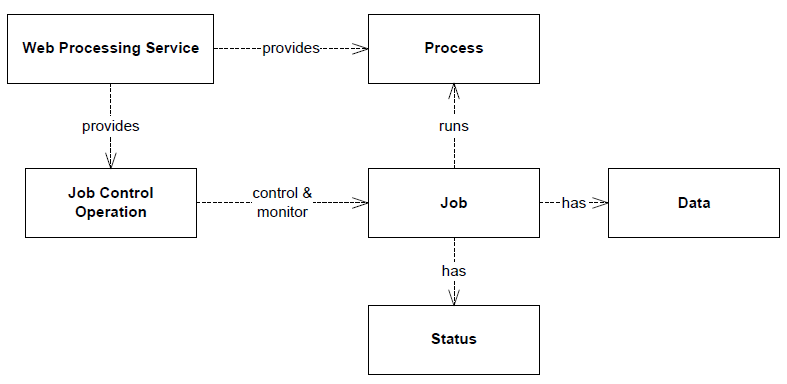
\includegraphics[width=1\linewidth]{UML/WPSmodel.png}
	\caption{Artifacts of the \ac{wps} service model \citep[p. 15]{GEO:OGC}}
	\label{fig:WPSmodel}
\end{figure}

\subsection{Get Capabilities}
All \ac{ogc} web services give an overview of what they have to offer using the so-called \texttt{GetCapabilities} request. The request can be made by taking the \ac{http} address of the \ac{wps} and adding: \url{service=wps&request=getcapabilities}. This returns a document with information about the service metadata, the basic process offerings, and available processes. Figure \label{fig:WPSmodel2} shows the model of this capabilities document. The service identification section of the document gives a description of the service, including the versions that it supports and potential fees or access constraints. The service provider section gives information about the organisation or people who maintain the \ac{wps} and also includes their contact information. The operations metadata lists the different requests that are implemented in this particular \ac{wps} and the \ac{http} addresses to which the GET and POST requests can be send to. The content section of the capabilities document provides an overview of the available process offerings. For every process an identifier, title and description are listed. Optionally an extensions section can be added that describes additional service capabilities. At the end of the document the language section lists the languages that are supported and the default language that is being used. An example of an capabilities document can be found in Appendix \ref{app:wpsCapabilities}  

\begin{figure}
	\centering
	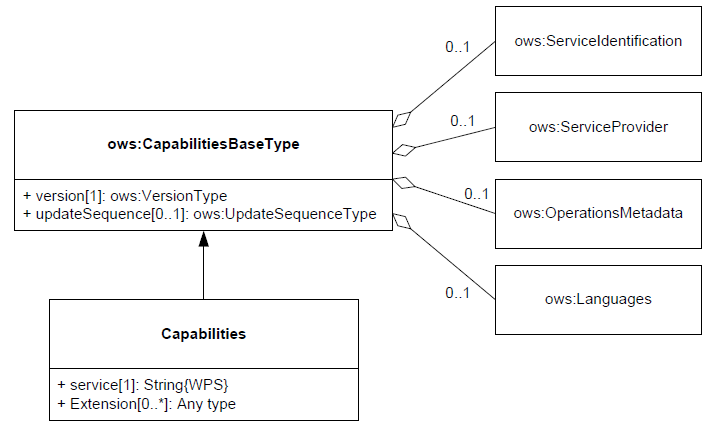
\includegraphics[width=1\linewidth]{UML/WPSmodel2.png}
	\caption{\ac{uml} model of WPS capabilities document \citep[p. 70]{GEO:OGC}}
	\label{fig:WPSmodel2}
\end{figure}

\subsection{Describe Process}
\begin{sloppypar}
A more detailed description of a process listed in the capabilities document of the \ac{wps} can be retrieved using the \texttt{DescribeProcess} request. This request requires the identifier of the process to be passed as a parameter. Optionally, a specific language can be requested for the response document (from the list of available languages in the capabilities document). The process description includes information about input parameters and output data, such as their identifiers, data type, mime types or default values. A describe sensor request can be made by putting the base address of the \ac{wps} and adding: \url{service=wps&version=1.0.0&request=describeprocess&identifier=an_identifier} where the version parameter should be in accordance with the supported version(s) from the capabilities document and the identifier should be taken from the process offerings section of the capabilities document. An example of an describe sensor response document can be found in Appendix \ref{app:wpsDescribe}  
\end{sloppypar}


\subsection{Execute}
A \ac{wps} process can be started using the \texttt{Execute} request. To make this request the \ac{http} address of the \ac{wps} is extended with: \url{service=wps&version=1.0.0&request=execute&identifier=GetSensors} where the version parameter should be in accordance with the supported version(s) from the capabilities document and the identifier should be taken from the process offerings section of the capabilities document. Additionally, the desired execution mode can be added to the request (synchronous, asynchronous or auto) as well as the desired output format (response document or raw data). By default the execution mode is set to `document'.

\begin{sloppypar}
	Depending on the individual requirements of the process, input parameters can be added using \url{&DataInputs=[parameterName1=value1;parameterName2=value2]}. The parameter names are defined in the describe process response document, as well as the allowed values for each parameter. There are two kinds of input parameters that can be put in a \texttt{Execute} request: literal and complex data inputs. Literal data inputs can be a string of characters in consisting of different data types (e.g. Double, Integer, String), a given value range, and associated units (e.g. meters, degrees Celsius) \citep[p. 36]{GEO:OGC}. 
\end{sloppypar} 

Complex data inputs are made for inputting complex vector-, raster- or other kind of data. This data can be inserted directly in the request or indirectly by referencing to a file. The process will then first retrieve this file from a remote server before running. A complex data input defines the allowed mime types that the process accepts.  

When the process finishes an execute response document is retrieved. This document has a process section with the identifier, title and abstract of the finished process. It also contains a status section with the time the process ended and whether it finished successfully. If any output data has been produced an `ProcessOutputs' section is created that contains the identifiers of the outputs and the corresponding data. An example of an execute response document can be found in Appendix \ref{app:wpsExecute}

\subsection{Other requests}
\ac{wps} processes can run synchronously or asynchronously. With a synchronous execution the connection with the client stays open until the process has finished. However, for processes that take longer to execute the asynchronous mode is better suited. The process will continue running after the connection has been closed. With a \texttt{GetStatus} request the client can check whether the process is still running. This request is structured the same as the execute request, but with the mode set to `status'. Once it has finished the \texttt{GetResult} request allows the client to retrieve the output data. The \texttt{Dismiss} request can be made to communicate to the server that the client is no longer interested in the results of a job. This job will then be cancelled and its output deleted. A job identifier is a required parameter for all three of these requests. 
